\subsection{Architecture and Processes}\label{subsec:architecture-and-processes}

% ---------------------------------------------------------------------------
% Architecture - Class Diagram
\begin{frame}
    \frametitle{Architecture - Class Diagram}
    \begin{figure}
        \centering
        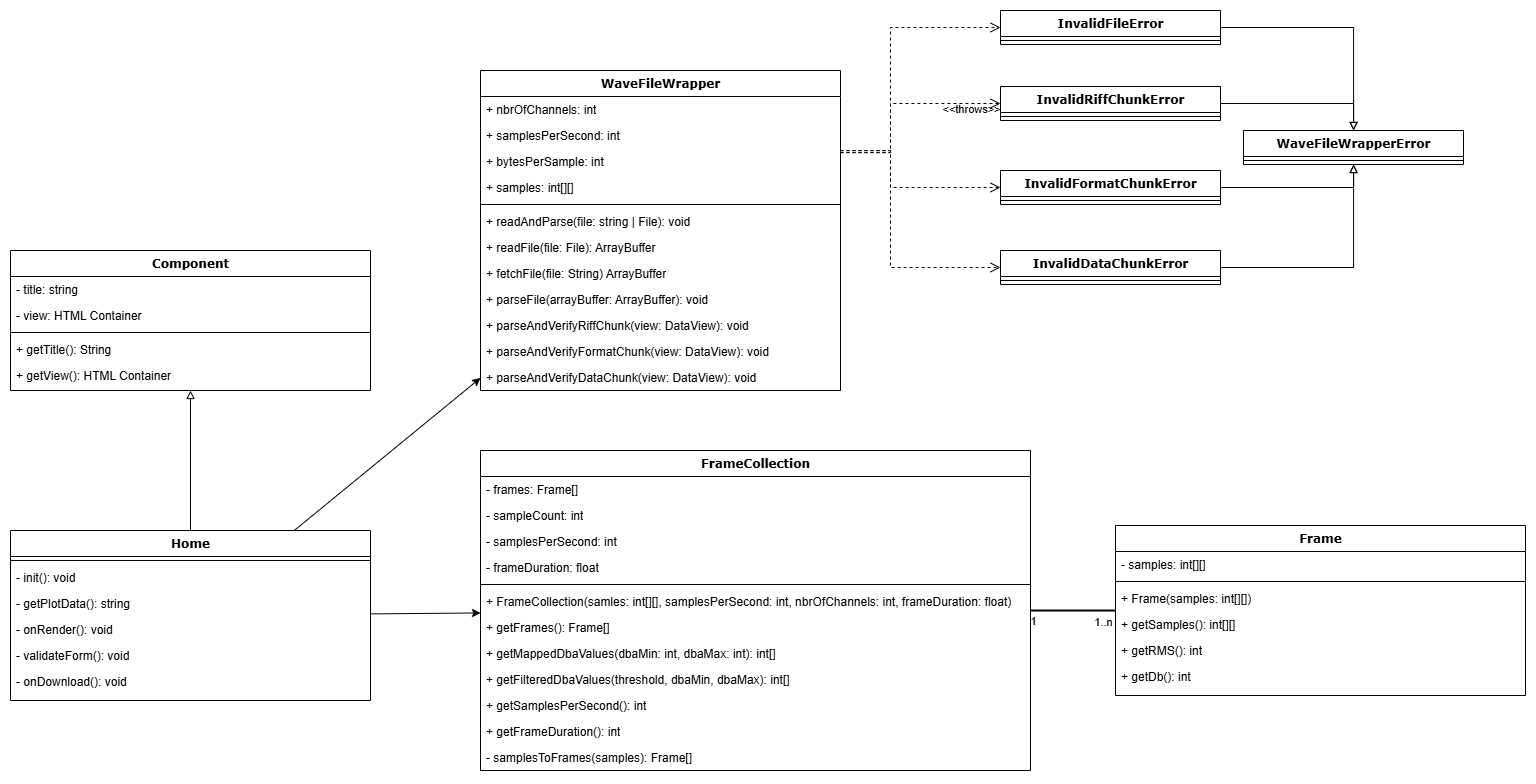
\includegraphics[width=0.95\textwidth]{../assets/class_diagram.png}
    \end{figure}
\end{frame}
% ---------------------------------------------------------------------------

% ---------------------------------------------------------------------------
% Architecture - SPA Techstack
\begin{frame}
    \frametitle{Architecture - SPA Techstack}
    \begin{columns}
        \column{0.5\textwidth}
            \begin{itemize}
                \item Vanilla JS SPA Framework (Web Programming Module) \\
                      ~
                \item Bootstrap CSS Framework \\ ~
                \item SwiftLaTeX in Browser WASM LaTeX rendering Library \\ ~
            \end{itemize}
        \column{0.5\textwidth}
            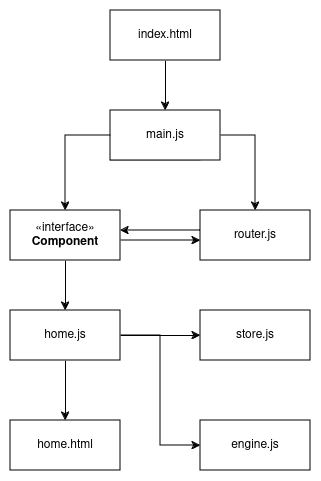
\includegraphics[width=0.6\textwidth]{../assets/spa_diagram.png}
    \end{columns}
\end{frame}
% ---------------------------------------------------------------------------

% ---------------------------------------------------------------------------
% Processes
\begin{frame}
    \frametitle{Processes}
    \begin{columns}
        \column{0.5\textwidth}
            \begin{enumerate}
                \item Read *.wav File
                \item Group samples into frames (duration of 300ms)
                \item Calculate root-mean-square (RMS) per frame
                \item Convert RMS dB values per frame
                \item Map the relative dB to absolute dB(A)
                \item Filter the resulting list of dB(A)
                \item Render PDF with dB(A) and user data
            \end{enumerate}
        \column{0.5\textwidth}
            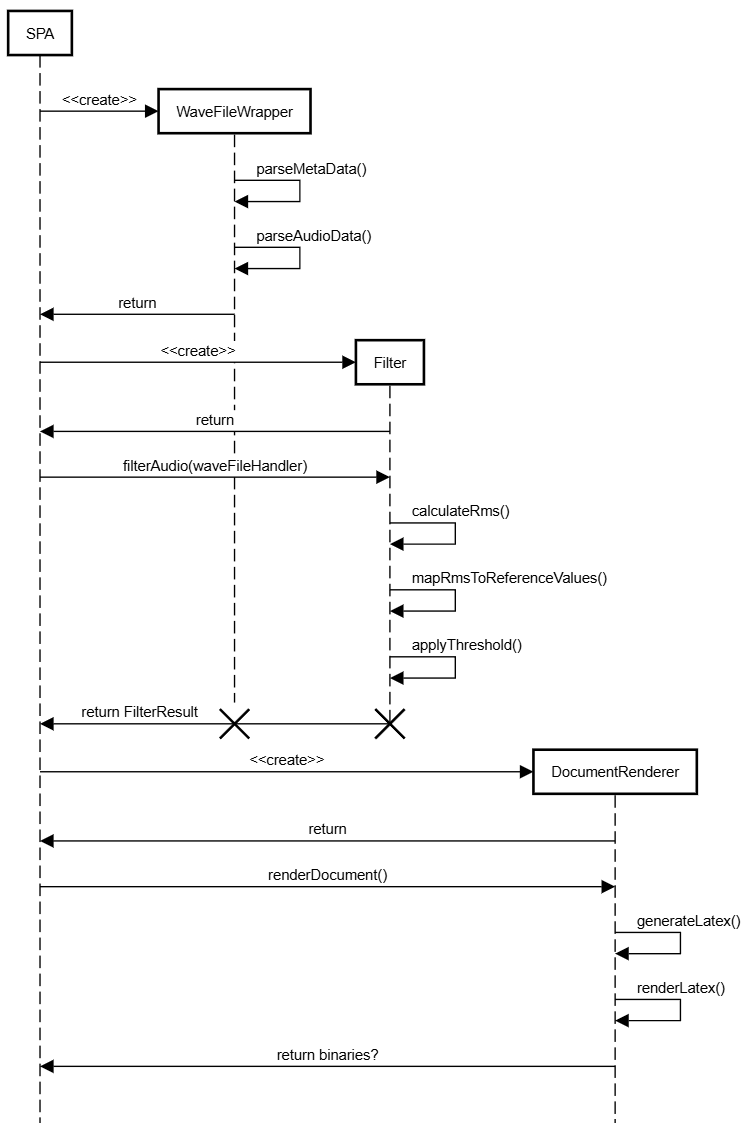
\includegraphics[width=0.6\textwidth]{../assets/sequence_diagram_from_wave_file_to_pdf.png}
    \end{columns}
\end{frame}
% ---------------------------------------------------------------------------

\subsection{Testing}\label{subsec:testing}

% ---------------------------------------------------------------------------
% Testing - Overview
\begin{frame}
    \frametitle{Testing - Overview}
    \begin{figure}[H]
        \centering
        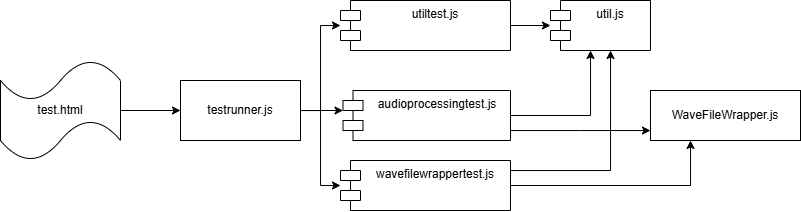
\includegraphics[width=1\textwidth]{../assets/overview_test_framework.png}
    \end{figure}
\end{frame}
% ---------------------------------------------------------------------------

% ---------------------------------------------------------------------------
% Testing - In action
\begin{frame}
    \frametitle{Testing - In action}
    \begin{figure}[H]
        \centering
        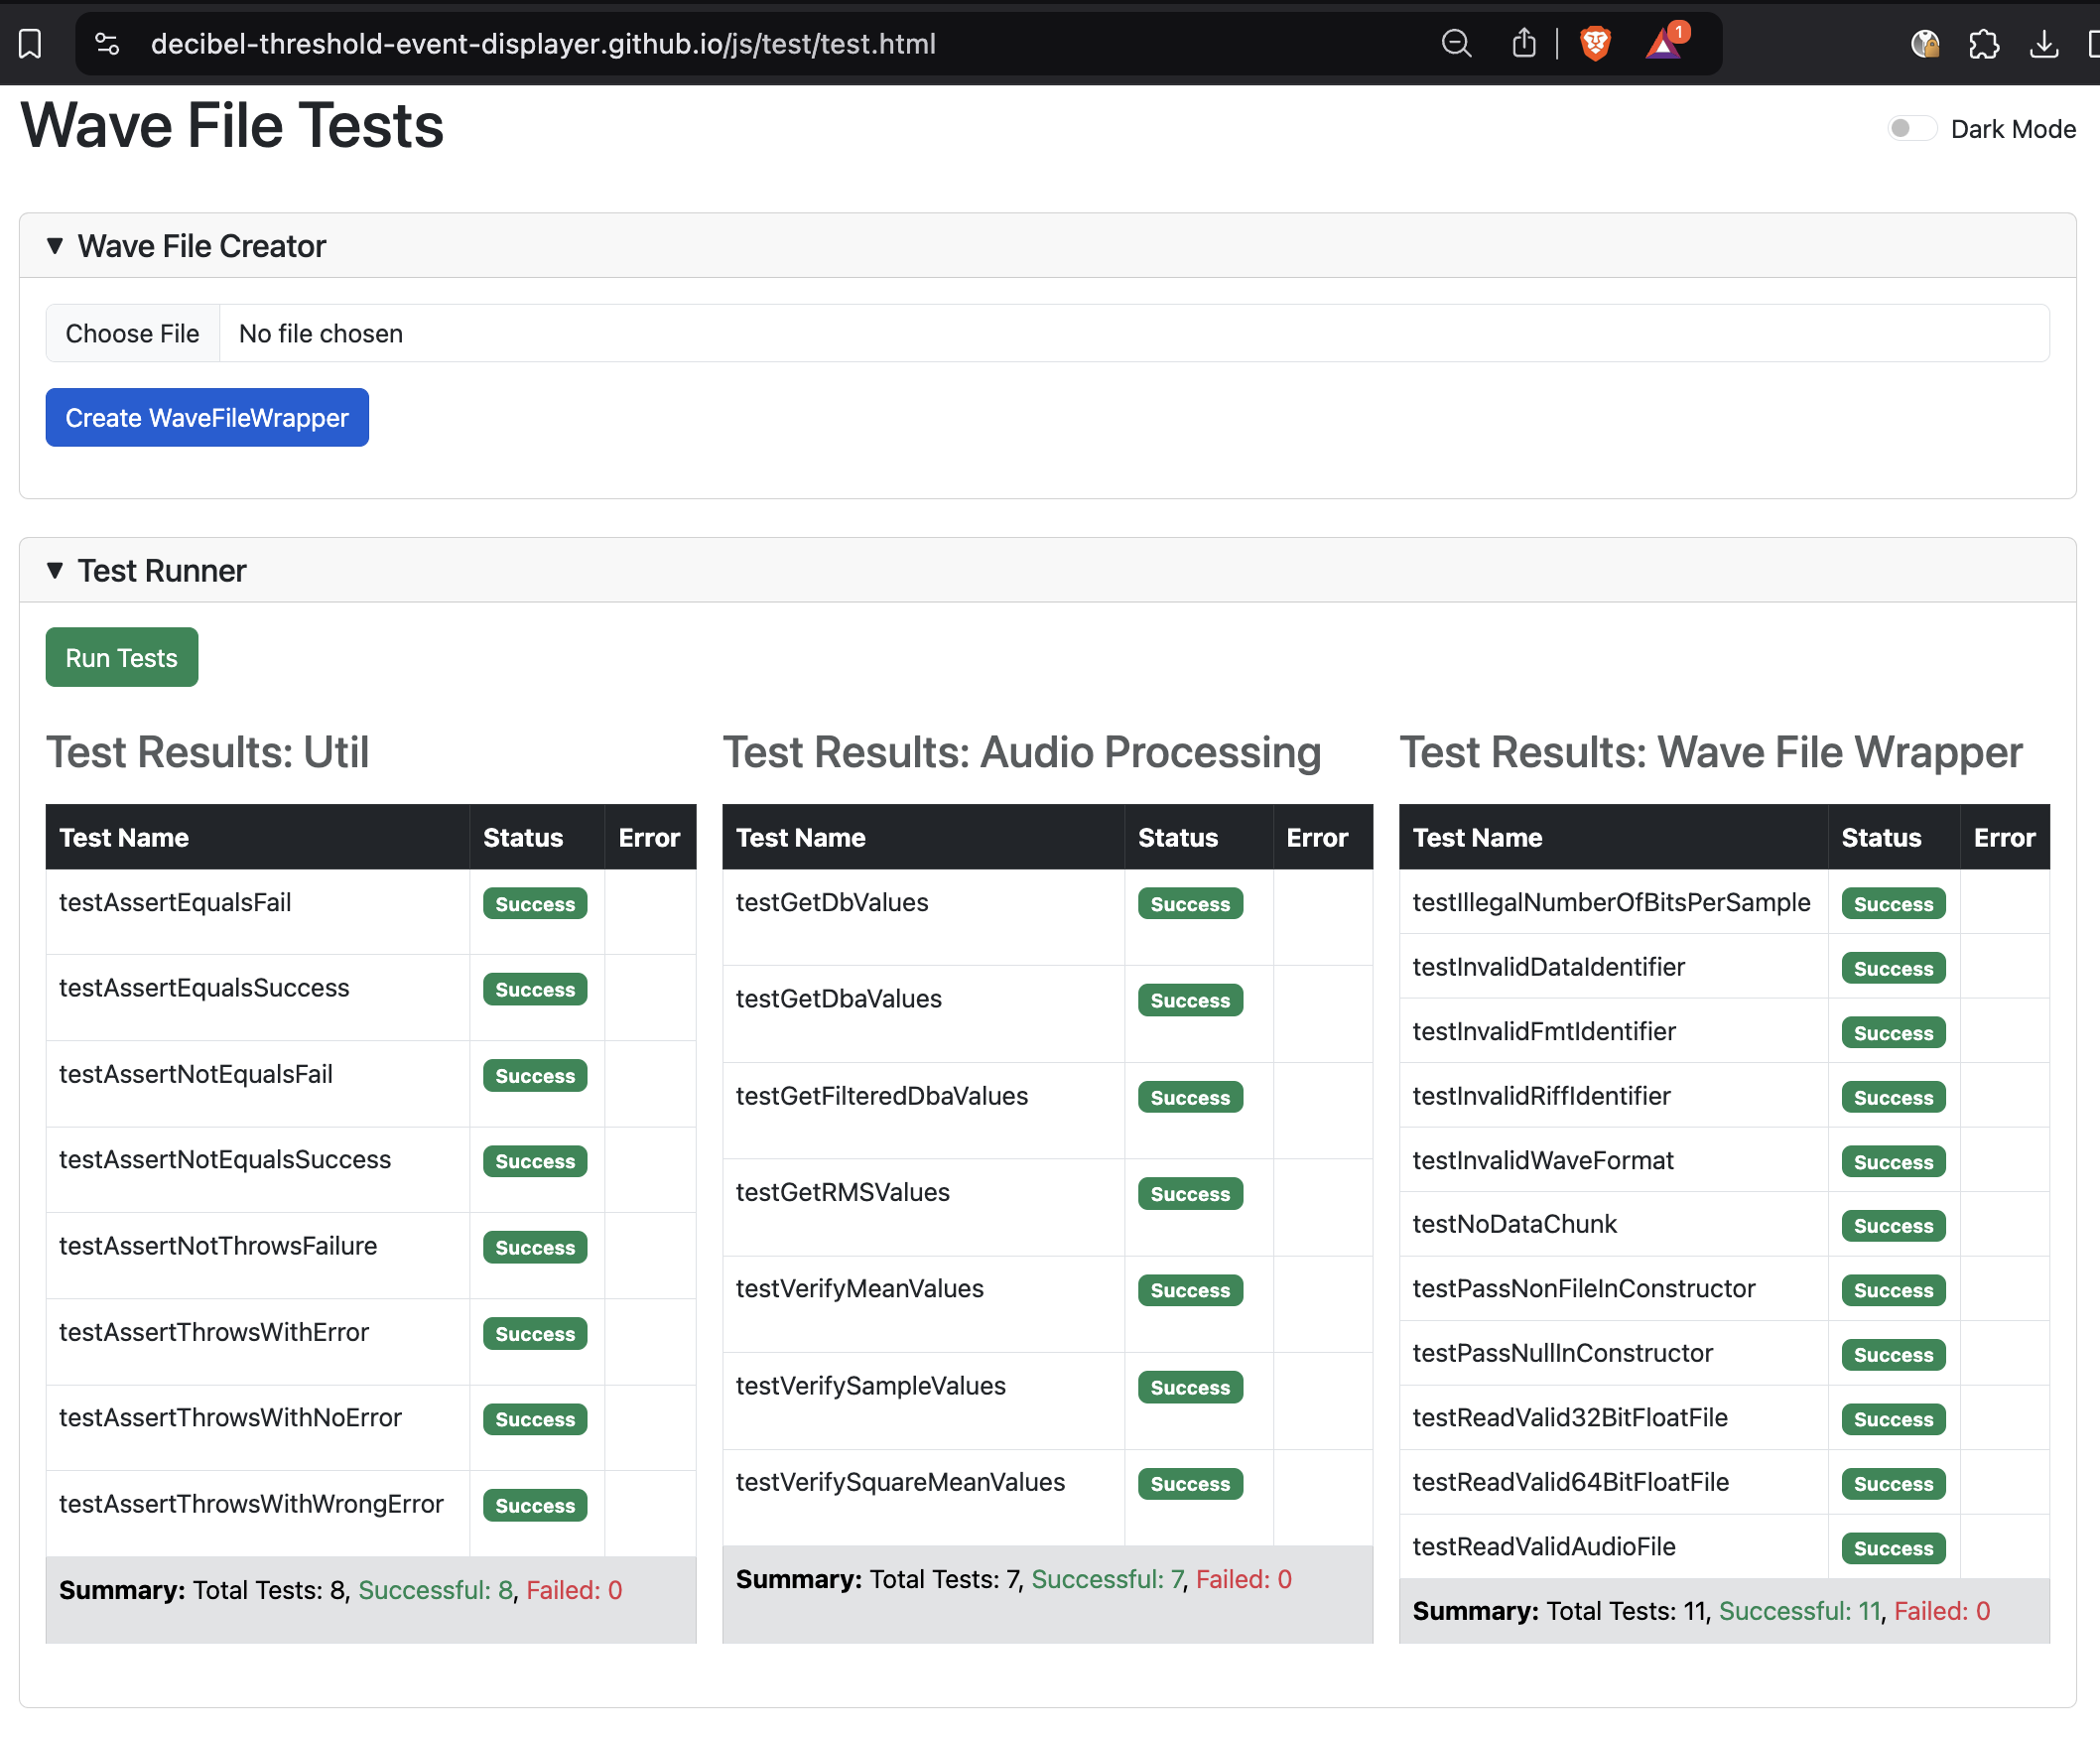
\includegraphics[width=0.6\textwidth]{../assets/js_test_framework_in_browser.png}
    \end{figure}
\end{frame}
% ---------------------------------------------------------------------------

\subsection{License and Privacy}\label{subsec:license-and-privacy}

% ---------------------------------------------------------------------------
% Privacy
\begin{frame}
    \frametitle{Privacy concerns}
    \begin{columns}
        \column{0.5\textwidth}
        \begin{itemize}
            \large
            \item No data is sent to the server, after the initial request
            \item From the Plot on the PDF the original Audio File cannot be recreated
        \end{itemize}
        \column{0.5\textwidth}
        \centering
        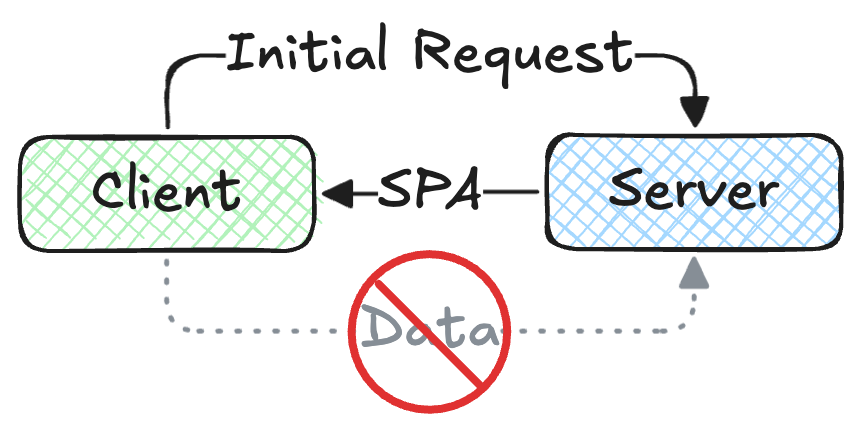
\includegraphics[width=1\linewidth]{../assets/privacy_illustrated.png}
    \end{columns}
    \hfill \break
    \hfill \break
    \textbf{
        The user does not get into legal trouble, \\
        using the application or the resulting PDF!
    }
\end{frame}
% ---------------------------------------------------------------------------

% ---------------------------------------------------------------------------
% License
\begin{frame}
    \frametitle{License}
    \begin{columns}
        \column{0.5\textwidth}
        Dependency Licenses:
        \begin{itemize}
            \large
            \item SwiftLaTeX: AGPL-3.0
            \item pgfplots: GPL-3.0
        \end{itemize}
        \hfill \break
        Resulting License:
        \begin{itemize}
            \large
            \item \textbf{GPL-3.0 licence (FLOSS)}
        \end{itemize}
        \column{0.5\textwidth}
        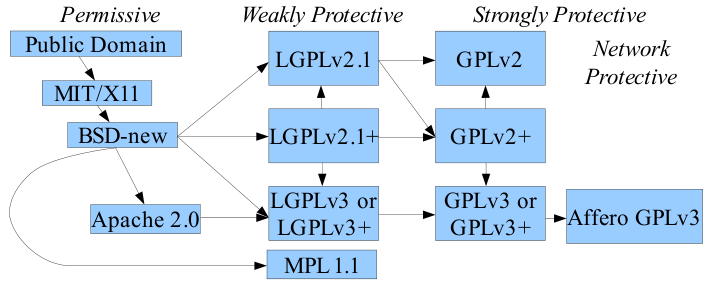
\includegraphics[width=1\linewidth]{../assets/floss-licenses.png}
    \end{columns}
    \hfill \break
    \hfill \break
    \hfill \break
    \hfill \break
    \hfill \break
    \hfill \break
    \small
    Image Source: https://dwheeler.com/essays/floss-license-slide.html
\end{frame}
% ---------------------------------------------------------------------------

\subsection{Deployment / Distribution}\label{subsec:deployment-and-distribution}

% ---------------------------------------------------------------------------
% Deployment / Distribution
\begin{frame}
    \frametitle{Deployment / Distribution}
    \begin{columns}
        \column{0.5\textwidth}
            \begin{enumerate}
                \large
                \item A dev pushes or merges code to the main branch
                \item GitLab automatically mirrors the repository to GitHub
                \item GitHub deploys automatically to GitHub Pages
                \item The Application is available under: \\
                      https://decibel-threshold-event-displayer.github.io/
            \end{enumerate}
        \column{0.5\textwidth}
            \centering
            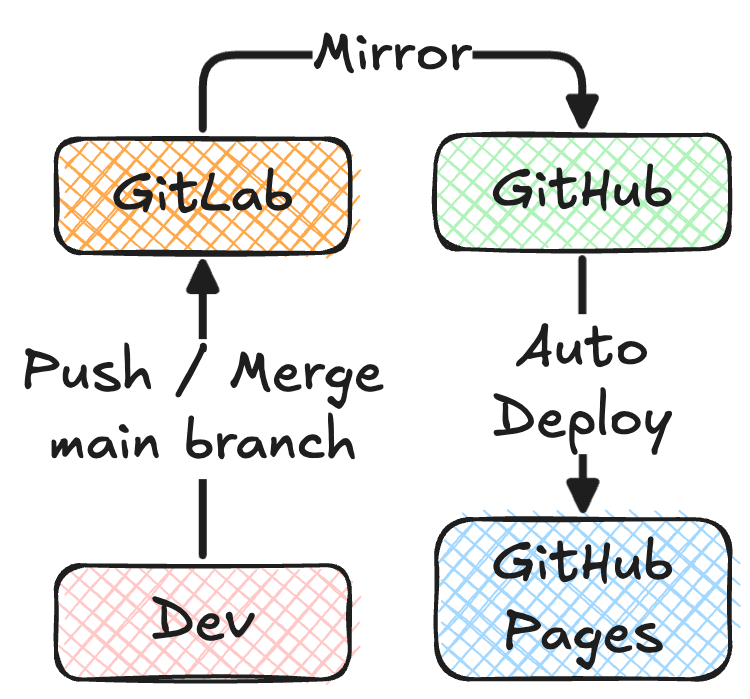
\includegraphics[width=1\linewidth]{../assets/deployment_and_distribution.png}
    \end{columns}
\end{frame}
% ---------------------------------------------------------------------------
